\documentclass[10pt,letterpaper]{article}
\usepackage[utf8]{inputenc}
\usepackage{amsmath}
\usepackage{amsfonts}
\usepackage{amssymb}
\usepackage{graphicx}

% Construct the basic page sizes
\oddsidemargin  0.0in
\evensidemargin 0.0in
\textwidth      6.5in
\headheight     0.25in
\topmargin      0.0in
\textheight=8.5in

\author{Darrel J. Conway\\Thinking Systems, Inc.}
\title{Building a GMAT Plug-in: A Walkthrough Using Visual Studio 2010}
\begin{document}
\maketitle
\begin{abstract}
This document walks a Visual Studio Windows developer through the process of building a plug-in module for the General Mission Analysis Tool (GMAT).  The procedure starts the reader from a predefined set of skeleton code available online, and shows the user how to configure that code to add a custom feature to GMAT.  The example plug-in used in this walkthrough writes information to the GMAT message window.

Appendices to the document describe the steps needed to configure the same code for use in Linux and Mac, and the procedure for setting up Visual Studio project files from scratch to build a GMAT plugin.  
\end{abstract}

The General Mission Analysis Tool (GMAT) is a spacecraft mission design and analysis tool that lets users model spacecraft trajectories using high fidelity physical models.  The tool provides capabilities for spacecraft trajectory propagation, maneuvering using impulsive or finite duration thruster firings, parameter targeting and optimization, and mission data modeling and analysis.  Additional capabilities can be added to GMAT by writing shared libraries that extend the core system functionality.  These plug-in modules have been used to add new optimizers, numerical integrators, atmospheric models, and event computations to GMAT.  Complex subsystem can also be added using the plug-in interfaces.  One example is the prototype estimation capabilities added to GMAT and released starting in 2011, which includes both batch least squares and extended Kalman filters, along with several simple and complex measurement models and a data simulator.  The Plug-in system was first presented at the 4th International Conference on Aerospace Tools and Techniques\cite{Madrid} and described in some detail in an earlier developer's document\cite{PluginDoc}.

In this document, I will walk new developers through the process of adding a plug-in module to GMAT.  The example used for this tutorial will add a new command to GMAT's Mission Control Sequence that writes data to the GMAT Message Window.  I'll begin by describing the basic configuration needed as a starting point, and then direct you to the files needed to work through the exercise.  Next we'll look at the desired functionality, and then use the starting files to add this functionality to GMAT.  Once the code compiles, we'll configure GMAT ti use the new plug-in, completing the lesson.

The instructions provided here assume you are building GMAT using Visual Studio 2010 on a Windows based computer.  Appendix A described the differences you will see if you build on Mac or Linux.  This lesson is driven from a core set of configuration files that set up the basic Visual Studio project settings for compilation.  Appendix B describes these settings for developers that want to build their project from scratch.

\section{Preparation}

In order to build a GMAT plug-in, you need a computer configured to build GMAT on the operating system you plan to use with your plug-in.  This document is aimed at developers working on Microsoft Windows, developing with Visual Studio 2010.  The development environment setup instructions are provided in a document in GMAT's repository on SourceForge\cite{vsSetup}.  You'll need to retrieve the source code and data files from that location in order to proceed.  The Plug-in code builds on code contained in GMAT's source files, so you need those files, arranged as described below, in order to proceed\footnote{The file arrangement and other setup requirements described here are needed regardless of your development platform.  Visual Studio specifics don't enter the discussion until I start describing the code in the next section.}.

\section{Configuration to Build a Plug-in}

The project files used for this walkthrough assume that you have a specific arrangement of source code files and dependencies.  The path data is entered in the Visual Studio project files using relative path information.  If you are using a different file arrangement, you'll need to make adjustments to the project file settings as described in Appendix~\ref{settings}.

Figure~\ref{files} shows the folder structure used in the instructions that follow.  You should already have the Gmat3rdParty folder and GmatDevelopment folder set up on your computer from when you configured it and built GMAT, following the instructions referenced in the preceding section.  We will now proceed to collect the files you need for this Walkthrough.  Those files are managed in the GMAT Plugins project at SourceForge.

\begin{figure}[htb]
\begin{center}
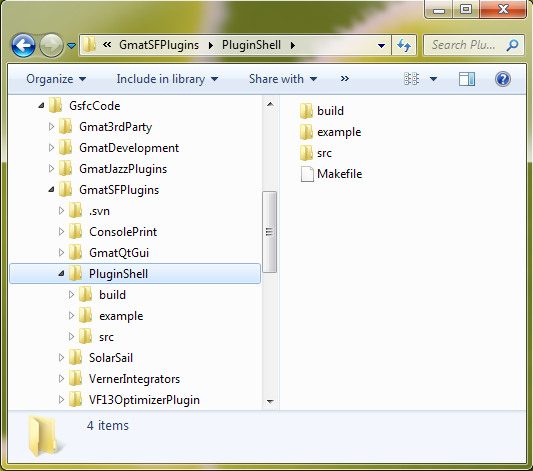
\includegraphics[scale=0.5]{images/FileStructure.png} 
\caption{\label{files}Folder Structure after Downloading Plugin Repository}
\end{center}
\end{figure}

\subsection{\label{settingUp}Retrieving and Setting Up the Files}

The code used in this tutorial can be downloaded from the GMAT Plugins repository at SourceForge.  The command line checkout of the entire plug-ins repository can be perfomed by changing directories to the desired location of the code (that is, to the folder containing your Gmat3rdParty and GmatDevelopment folders), and then executing this command:
\begin{quote}
\begin{verbatim}
svn checkout svn://svn.code.sf.net/p/gmatplugins/code/trunk GmatSFPlugins
\end{verbatim}
\end{quote}
\noindent This command places all of the projects available in the GMAT Plugins repository on your machine.  The code we use for this tutorial is found in the folder named \texttt{PluginShell{\textbackslash}src}.  We will work with a copy of the files contained in that folder, so that the project files and associated source remain in an unconfigured stat in case you want to start a new plug-in from them after completing this exercise.  To finish preparing to work:

\begin{enumerate}
\item Create a new folder named SamplePlugin in the folder containing GmatDevelopemnt and Gmat3rdParty.
\item Copy the PluginShell folder into the SamplePlugin folder.
\item Open the example folder in your SamplePlugin folder, and copy the command folder from that location into the SamplePlugin{\textbackslash}src folder. 
\end{enumerate} 

\noindent When you are finished with this step, your folders should be arranged as shown in Figure~\ref{folderConfig} shows the folder arrangement after moving the command folder.

\begin{figure}[htb]
\begin{center}
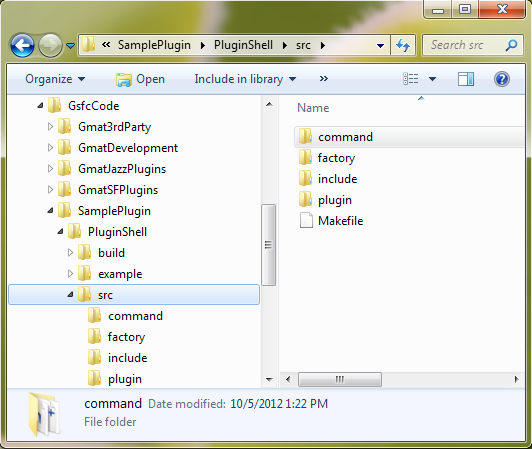
\includegraphics[scale=.5]{images/FolderConfiguration.png}
\caption{\label{folderConfig}Folder Arrangement for the Walkthrough}
\end{center}
\end{figure}

\noindent We are now ready to begin defining and building our plug-in.

\section{Defining the Desired Functionality}

When GMAT runs a mission, it provides the user with information about progress in the run in a window at the bottom of the main GMAT window.  The panel that receives this information is called the Message Window.  Figure~\ref{msgWindow} shows this window.

\begin{figure}[htb]
\begin{center}
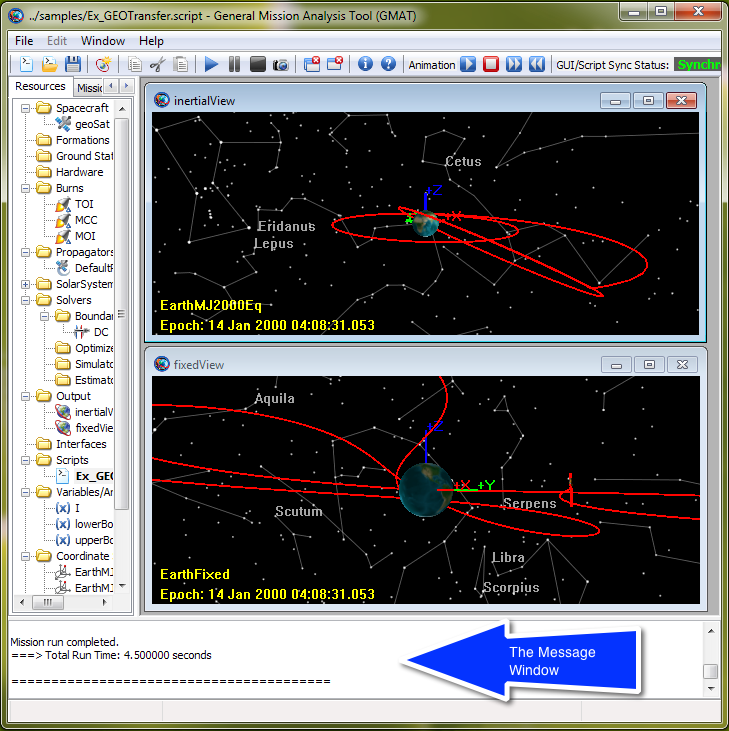
\includegraphics[scale=.5]{images/TheMessageWindow.png}
\caption{\label{msgWindow}The Message Window}
\end{center}
\end{figure}

\noindent GMAT defines a static class named MessageInterface which is used to send text to this window using a syntax similar to the C printf function.  A call to write to the message window looks like this:

\begin{quote}
\begin{verbatim}
double myFloat = 3.141592653589793
MessageInterface::ShowMessage("Here is an example showing pi: %lf\n",
      myFloat);
\end{verbatim}
\end{quote}

\noindent When this code executes, the scripted line appears in teh message window.  The code that we'll use in the plug-in described here uses this framework to create a new GMAT Mission Control Sequence command that wraps this interface into a scriptable instruction for your GMAT missions.  When we are done, you'll be able to pass strings, variables, and some object parameters to the command, which will then write their values to the message window.  The command syntax for this is scripted in GMAT as follows:

\begin{quote}
\begin{verbatim}
Create String hi

%----------------------------------------
%---------- Mission Sequence
%----------------------------------------
BeginMissionSequence;

hi = 'Hello, VS2010 Plugin Developers!';
ConsolePrint hi
\end{verbatim}
\end{quote}

\noindent Let's begin setting Visual Studio up to build the plugin that makes this work.

\section{Setting Up Visual Studio 2010}

Set up Visual Studio 2010 (VS2010) using solution and project files are part of the code we copied from the plugins repository earlier by following these steps:

\newcounter{saveenum}
\begin{enumerate}
\item Open Visual Studio 2010.
\item From the File menu, select Open \textgreater Project/Solution...
\item Select the PluginShell.sln solution file from your SamplePlugin{\textbackslash}PluginShell{\textbackslash}build{\textbackslash}VS2010 folder and select the Open button.  
\setcounter{saveenum}{\value{enumi}}
\end{enumerate}

\noindent This opens the solution and project files in Visual Studio.  First we need to set the developemnt environment to build the plug-in library with setting compatible with the standard GMAT build.  We want to set the system to build a release version of the library using Microsoft's 32-bit compiler.  These settings are made using comboboxes (that is, drop-down selections) at the top of the VS2010 window, just below the menu bar.  In the first combobox, select Release.  In the second combobox, select Win32.  When you are finished, your configuration should look like Figure~\ref{VS2010PlatformSettings}.

\begin{figure}[htb]
\begin{center}
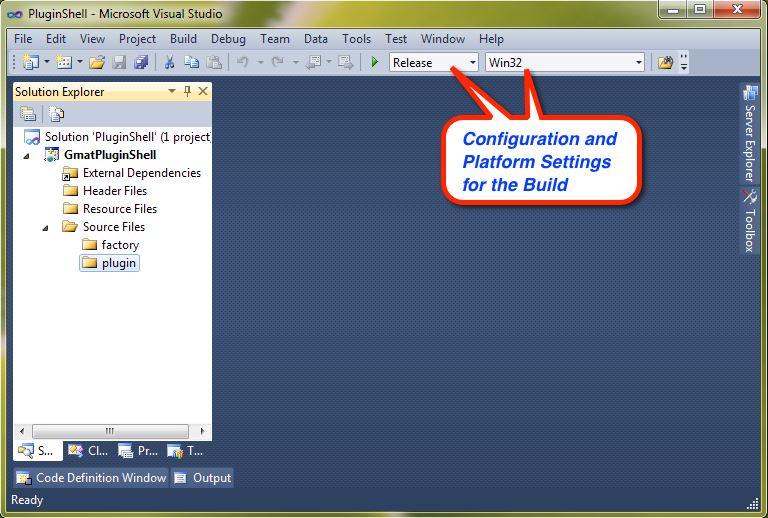
\includegraphics[scale=.5]{images/VS2010BuildSettings.png}
\caption{\label{VS2010PlatformSettings}Selecting the Configuration and Platform for the Build}
\end{center}
\end{figure} 

If you look closely at Figure~\ref{VS2010PlatformSettings}, you'll see that the factory and plugin folders in the project do not contain any files, and that there is no command folder in teh project.  That is because the project in its configuration in the repository does not yet contain any source code file references.  We need to tell it about the code that we will be compiling.  We set the new folder up as a ``filter'' in VS2010, and the file references using Windows Explorer:

\begin{enumerate}
\setcounter{enumi}{\value{saveenum}}
\item In the Solution Explorer on the left side of the VS2010 window, right click on the ``Source Files'' label and select Add \textgreater New Filter.  A new folder is added to the project tree named ``NewFilter1'.  
\item Change the filter's name to ``command''.
\item If VS2010 is running full screen on your computer, select the ``Restore Down'' button to shrink it into a window that you can place next to another window.
\item Open Windows Explorer, and size it so that you can see both the Windows Explorer contents and the VS2010 Solution Explorer.
\item Navigate in Windows Explorer to your PluginShell{\textbackslash}src{\textbackslash}include folder.  You should see a file named SampleDefs.hpp.
\item Drag the SampleDefs.hpp file from Windows Explorer to the VS2010 Solution Explorer, and drop it into the GmatPluginShell{\textbackslash}Header Files folder.
\item Navigate in Windows Explorer to your PluginShell{\textbackslash}src{\textbackslash}factory folder.  You should see two files in this folder.
\item Select both files, and drag them from Windows Explorer into the VS2010 Solution Explorer, dropping them into the GmatPluginShell{\textbackslash}Source Files{\textbackslash}factory folder.
\item Repeat this procedure for the files in the PluginShell{\textbackslash}src{\textbackslash}command and PluginShell{\textbackslash}src{\textbackslash}plugin folders.
\end{enumerate}

\noindent When you have finished, your VS2010 Solution Explorer should match the one shown in Figure~\ref{VS2010WithFiles}.

\begin{figure}[htb]
\begin{center}
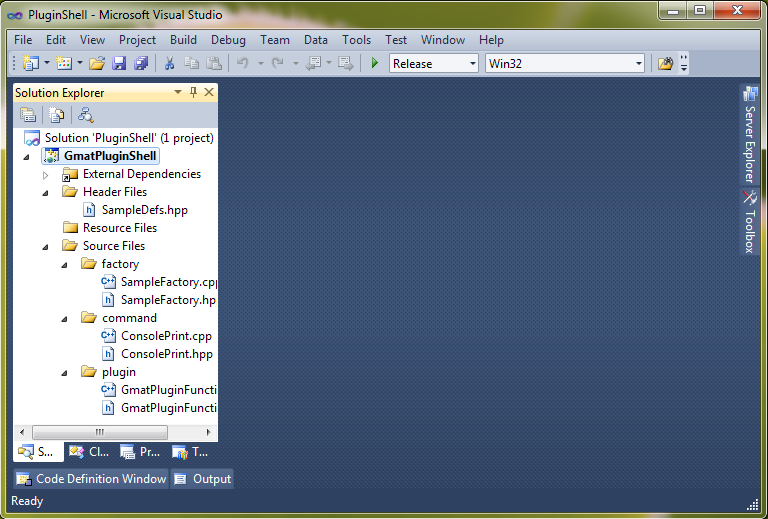
\includegraphics[scale=.5]{images/VS2010WithFiles.png}
\caption{\label{VS2010WithFiles}VS2010 with the Plug-in File References Set}
\end{center}
\end{figure} 

\section{Coding the Plug-in}

GMAT plug-ins consist of three distinct pieces: the code that implements the new functionality, a set of Factory subclasses that are used to build new GMAT components coded into the plug-in, and a set of C style interfaces GMAT uses to learn about and access the plugin contents.  The following sections describe each of these elements.

\subsection{Coding the New Functionality}

The lines in the Mission Control Sequence that define the actions taken when you run a mission are implemented through classes derived the the GmatCommand class.  GmatCommand, in turn, is derived from GmatBase, the core class for all of the objects in the model describing the user's mission.  The ConsolePrint command we are building into the plug-in is derived from GmatCommand.  Source code for this command is in the command folder you copied into the src folder in Section~\ref{settingUp}.

Open the file src{\textbackslash}command{\textbackslash}ConsolePrint.hpp in a text editor.  Near the top of that file you'll find the lines

\begin{quote}
\begin{verbatim}
...
#include "SampleDefs.hpp"
#include "GmatCommand.hpp"
#include "MessageInterface.hpp"

/** 
 * Example functionality used in the plug-in walkthrough document.
 *
 * This command adds functionality to GMAT that enables scripting of text to the
 * GMAT Message Window.
 */
class SAMPLE_API ConsolePrint : public GmatCommand
{
...
\end{verbatim}
\end{quote}

There are two things I want to point out in these lines.  First, the class definition includes a preprocessor macro, SAMPLE{\_}API.  This macro is used to specify the Windows dynamic link library import and export interfaces provided for the class\footnote{Developers writing code for Linux and Mac do not need this macro for their platform.  However, since GMAT is written to be cross-platform compatible with Windows, setting up this piece from the start will simplify porting code to run on Windows if that ever becomes necessary.}.  Every class that is exposed between GMAT modules (that is, between two shared libraries, or between a shared library and a GMAT executable) needs to identify themselves.  This specification is done for the ConsolePrint command using the SAMPLE{\_}API macro.  

The second item to look at is the include line at the start of the listing above.  The file SampleDefs.hpp is contained in the src{\textbackslash}include folder.  That file defines the SAMPLE{\_}API macro in a manner that defines it for all of the platforms GMAT supports.  This is done by wrapping the macro definition inside of a set of nested macros, shown here in an abbreviated form:

\begin{quote}
\begin{verbatim}
#ifdef _WIN32  // Windows
   #ifdef _DYNAMICLINK  // Only used for Visual C++ Windows DLLs
      #ifdef SAMPLE_EXPORTS
         #define SAMPLE_API __declspec(dllexport)
      #else
         #define SAMPLE_API __declspec(dllimport)
      #endif
   #endif
#endif //  End of OS nits

#ifndef SAMPLE_API
   #define SAMPLE_API
#endif
\end{verbatim}
\end{quote}

\noindent (The full definition in SampleDefs.hpp includes other pieces needed for working with the Standard Template Library string classes in Windows DLL's.  If you'd like to see the full code, open SampleDefs.hpp in VS2010 by double clicking on teh file name we set in the VS2010 Solution Explorer.)  When we build the plug-in, we'll define the preprocessor macros {\_}DYNAMICLINK and SAMPLE{\_}EXPORTS, which will give the compiler the correct definitions to allow export of the ConsolePrint class.

The code implementing the ConsolePrint command is in the src{\textbackslash}command{\textbackslash}ConsolePrint.cpp file.  If you are interested in how the command performs its function, refer to the code found there.  For now, we are interested in the mechanics of exposing that functionality to GMAT, and will use the ConsolePrint command code without making any changes.  

All model components that a user defines through a script are managed in GMAT using a class derived from GMAT's Factory class.  We will configure the factory for the ConsolePrint command next.  

\subsection{The Plug-in Factory}

\begin{figure}[htb]
\begin{center}
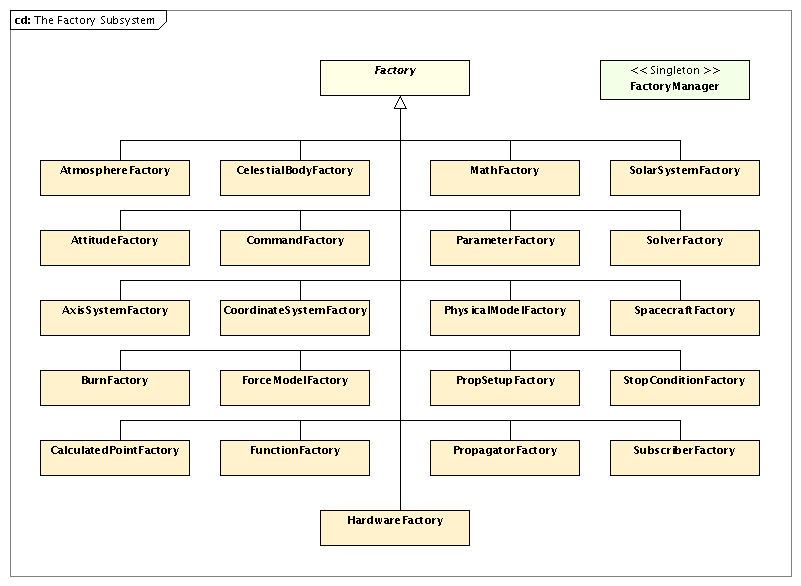
\includegraphics[scale=0.5]{images/TheFactorySubsystem.png}
\caption{\label{Factories}GMAT's Factory Types}
\end{center}
\end{figure}

In GMAT, objects that the user scripts are created from classes through a call to a GMAT Factory.  Each Factory accesses the constructor of one or more classes to create objects of a specific core type.  Most of the core types GMAT supports are shown in Figure~\ref{Factories}.  Since the ConsolePrint class is a GmatCommand, we need to configure a Command Factory to create instances of the class.  We'll do this in the SampleFactory code we added to VS2010 earlier.

\begin{enumerate}
\item Open VS2010 if it is not already open, and load the GmatPluginShell solution.
\item Open the header file SampleFactory.hpp by double clicking on its node in the Solution Explorer.
\item Find the following lines in the header file:
\begin{quote}
\begin{verbatim}
//virtual GmatCommand*     CreateCommand(const std::string &ofType,
//                                       const std::string &withName = "");
\end{verbatim}
\end{quote}
\item Uncomment these lines.
\item Save the file.
\setcounter{saveenum}{\value{enumi}}
\end{enumerate}

The factory we are configuring here is used to create instances of the ConsolePrint command object.  Since that object was derived from GMAT's GmatCommand class, we need to be sure that the factory has a method for creating GmatCommand objects.  That is what we have done by declaring that our SampleFactory has a CreateCommand method.  In GMAT, each factory can create one and only one type of base object.  In this case, we are creating commands from our factory, so the SampleFactory can only create command objects.  If we had several different types of commands, we could have this single factory support all of the commands that we were adding to GMAT.  For now, though, we are only interested in adding the ConsolePrint command.  We have identified the new method that we need to support the command, so now we need to implement it:

\begin{enumerate}
\setcounter{enumi}{\value{saveenum}}
\item Open the SampleFactory.cpp file.  Add the following code to the bottom of the file (you'll find this code already in place there, commented out, so all you need to do is uncomment it):
\begin{quote}
\begin{verbatim}
GmatCommand* SampleFactory::CreateCommand(const std::string &ofType,
                                     const std::string &withName)
{
   // This is how you'd implement creation of a ConsolePrint command 
   if (ofType == "ConsolePrint")
      return new ConsolePrint();
   // add more here .......

   return NULL;   // doesn't match any type of Command known by this factory
}
\end{verbatim}
\end{quote}
\setcounter{saveenum}{\value{enumi}}
\end{enumerate}

This code performs the work required of the factory by creating and returning a new ConsolePrint command to GMAT when the method is invoked with the input string ``ConsolePrint''.  GMAT's Factory Manager learns about the types of objects that a factory can create though a parameter that is set when the factory is created.  It also learns the scripted names of the objects available in the factory by obtaining an array of names.  We configure these items next:

\begin{enumerate}
\setcounter{enumi}{\value{saveenum}}
\item At the top of SampleFactory.cpp, we need to identify the core type supported by the factory.  Thar piece of the code is set correctly for command factories, in these lines:
\begin{quote}
\begin{verbatim}
SampleFactory::SampleFactory() :
   Factory           (Gmat::COMMAND)
{
...
\end{verbatim}
\end{quote}
so we don't need to make a change for this part of the code.  If you were adding a different type -- for example, a force used in the force model -- you would change the Gmat::COMMAND parameter to the correct type (for instance, Gmat::PHYSICAL{\_}MODEL for a new force).
\item If you continue reading the default constructor, you'll find the list of cratable objects for the factory: 
\begin{quote}
\begin{verbatim}
...
   if (creatables.empty())
   {
      // Replace the SampleClass string here with your class name.  For multiple 
      // classes of the same type, push back multiple names here
      creatables.push_back("SampleClass");
   }
}
\end{verbatim}
\end{quote}
Replace the string ``SampleClass'' with the script name for our new command, ``ConsolePrint''.
\item The same string appears twice more in the code setting the creatables array; replace those occurances as well.
\item Finally, we need to add the header file for the ConsolePrint command to the include list for the factory.  Near the top of the file, replace the include statement
\begin{quote}
\begin{verbatim}
#include "SampleClass.hpp"
\end{verbatim}
\end{quote}
with the line
\begin{quote}
\begin{verbatim}
#include "ConsolePrint.hpp"
\end{verbatim}
\end{quote}
\setcounter{saveenum}{\value{enumi}}
\end{enumerate}

TYhis completes configuration of the factory we need for the walkthrough.  In production code, you would remove the extra commented out methods prototypes in the header file, rename the factory class itself to something more informative -- perhaps PrintFactory for this example -- and polish the code a bit more.  

\subsection{The Plug-in Interfaces}

Before we can compile, we need to fill in information used by GMAT when loading the plug-in.  This step us performed in the code in the plugin folder.  GMAT defines two interfaces that we need to adapt to our new code.  Open the GmatPluginFunctions.hpp file in VS2010 to see these interface functions.  The code we need to change is the first two functions in the extern ``C'' block:

\begin{quote}
\begin{verbatim}
extern "C"
{
   Integer    SAMPLE_API GetFactoryCount();
   Factory    SAMPLE_API *GetFactoryPointer(Integer index);
   void       SAMPLE_API SetMessageReceiver(MessageReceiver* mr);
};
\end{verbatim}
\end{quote}

GMAT calls these functions when it loads a Plug-in during start up.  Since they are called from an external program -- in this case, the Moderator in GMAT's main library, libGmatBase -- the functions include the DLL import/export SAMPLE{\_}API directive described above.  (Note that the Factory also had this macro in the class definition, since the factory is also accessed externally.)  The methods themselves are straightforfard.  The GetFactoryCount method returns an integer indicating how many classes derived from Factory are in the plug-in.  We have a single factory, so the default code (found in GmatPluginFunctions.cpp):

\begin{quote}
\begin{verbatim}
   Integer GetFactoryCount()
   {
      // Update this line with the total number of factories you support:
      return 1;
   }
\end{verbatim}
\end{quote}

is sufficient for our needs.  The second function returns a pointer to a Factory object.  If the plug-in contains multiple factories, the input parameter is used to identify which factory is needed.  Im out case, there is onle one factory, accessed as Factory number 0 (since C indexes from zero by default).  The default factory name is ``SampleFactory'' in this code, so we don't need to make any changes to the default implementation here either:

\begin{quote}
\begin{verbatim}
   Factory* GetFactoryPointer(Integer index)
   {
      Factory* factory = NULL;

	  // Update this code with your factories, one index per factory
      switch (index)
      {
         case 0:
            factory = new SampleFactory;
            break;
            
         default:
            break;
      }

      return factory;
   }
\end{verbatim}
\end{quote}

Finally, we need to be sure that the SampleFactory header file is included in order for this code to compile.  Since the line

\begin{quote}
\begin{verbatim}
#include "SampleFactory.hpp"
\end{verbatim}
\end{quote}

\noindent occurs near the top of the file, the code should be ready for use.

\section{Compiling and Running}

All of the coding for the plug-in is now complete.  However, if you try to build the project by right clicking on teh project node and selecting ``Build'' (go ahead and do this!), you'll find that the project cannot build.  The problem is reported in the VS2010 message window:

\begin{quote}
\begin{verbatim}
1>------ Build started: Project: GmatPluginShell, Configuration: Release Win32 ------
1>Build started 10/8/2012 3:36:35 PM.
...
1>ClCompile:
1>  SampleFactory.cpp
1>..\..\src\factory\SampleFactory.cpp(26): fatal error C1083: Cannot open include file:
 'ConsolePrint.hpp': No such file or directory
1>
1>Build FAILED.
\end{verbatim}
\end{quote}

The issue is that when we added the source code for the ConsolePrint command, we did not add the path for that code to the VS2010 C++ project file.  We'll do that now:

\begin{enumerate}
\item Right click on the GmatPluginShell node in the VS2010 Solution Explorer, and select ``Properties'' from the dialog that pops up.  (In default VS2010 setups, this entry is at the bottom.  It might not be at the bottom if you have added any VS2010 add-on libraries.)  The Property Pages dialog will open.
\item In the Configurations combobox in the upper left side of the panel, set the confiration to ``All Configurations''. 
\item On the left side of the Property Pages dialog, select the C/C++ | General setting.  (You may need to click on the arrow next to C/C++ entry to see this option.)
\item The topmost entry on the panel should be ``Additional Include Directories''.  Click on the downwards pointing arrow at the right side of the list of include directories (see Figure~\ref{IncludeLoc}, and select {\textless}Edit...{\textgreater}. 
\begin{figure}[htb]
\begin{center}
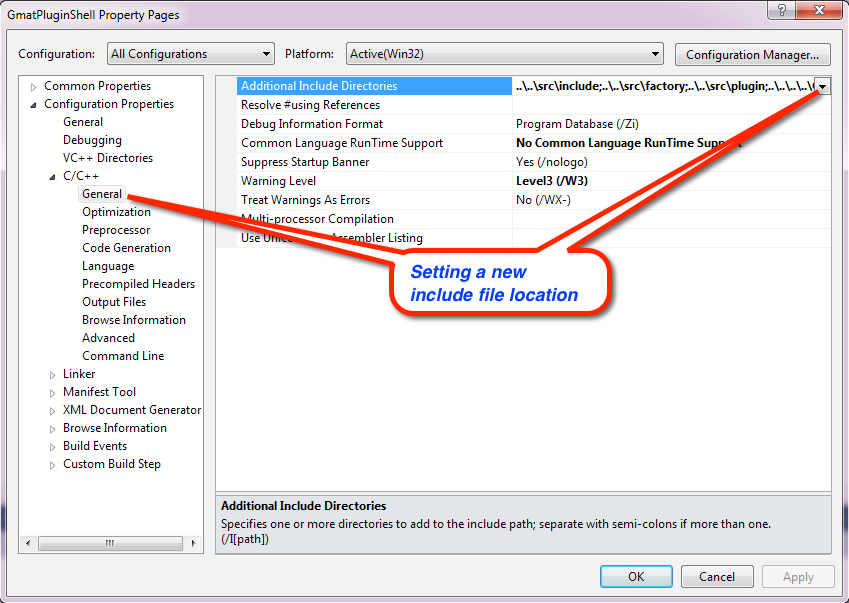
\includegraphics[scale=0.5]{images/SettingIncludeLocation.png}
\caption{\label{IncludeLoc}Adding a new include file folder}
\end{center}
\end{figure}

\item A dialog will appear showing the list of folders searched when the compiler needs to find a specified header.  We are going to add an entry to this list.
\item Select the line that reads ``..{\textbackslash}..{\textbackslash}src{\textbackslash}factory'', and press the control (Ctrl) and Insert kys simultaneously on your keyboard to insert a new line.
\item Add the line ``..{\textbackslash}..{\textbackslash}src{\textbackslash}command''
\item Apply the change by pressing the OK button.
\item Press the OK button on the Property Pages dialog to apply the changes to the project.
\end{enumerate}

Now try compiling the project again.  It should build and create a new library in your GMAT project folder.  Check to see if the file libSamplePlugin.dll is in your GmatDevelopment{\textbackslash}application{\textbackslash}plugin folder.  If so, the project built correctly and you are ready to configure GMAT to use the plugin.

\begin{enumerate}
\item Open your GMAT startup file (GmatDevelopment{\textbackslash}application{\textbackslash}bin{\textbackslash}gmat{\_}startup{\_}file.txt) in a text editor.
\item Add the line
\begin{quote}
\begin{verbatim}
PLUGIN                 = ../plugins/libSamplePlugin
\end{verbatim}
\end{quote}
\noindent to the list of plugin modules in the file.
\item Save the file.
\end{enumerate}

Now start GMAT.  If you select the Mission tab and right click on the top node, then select Append\textgreater, you'll see the ConsolePrint command in the list of commands available for use in teh Mission Control Sequence.   Finally, if you enter this script into GMAT:
 
\begin{quote}
\begin{verbatim}
Create String hi
BeginMissionSequence;
hi = 'Hello, VS2010 Plugin Developers!';
ConsolePrint hi
\end{verbatim}
\end{quote}

\noindent and run it, you'll see that the ConsolePrint command works as desired (see Figure~\ref{Results}).

\begin{figure}[htb]
\begin{center}
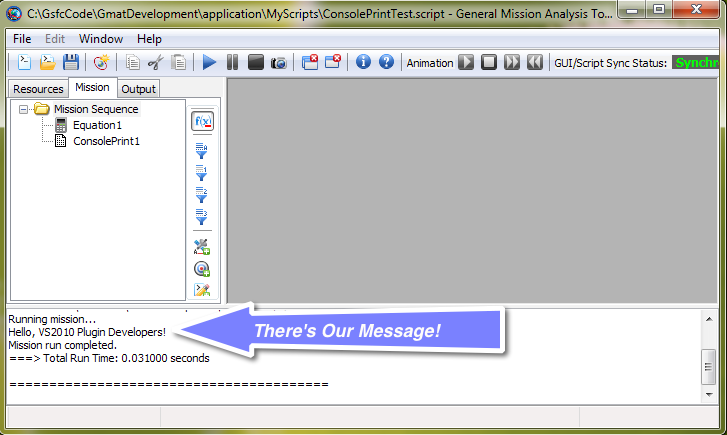
\includegraphics[scale=0.54]{images/FinalOutput.png}
\caption{\label{Results}Results of Running with teh ConsolePrint Command}
\end{center}
\end{figure}
 
\appendix
\section{Mac and Linux Configuration}

Configuration and build settings on the *nix platforms is made using gcc make files.  A sample set of make files is included in the code checked out from the plugins repository.  Each platform has a build environemtn file that is included from the make files, and used to set platform specific information.  This file, SampleEnv.mk, should be copied into your src folder and then edited to identify the locations of the GMAT code and otehr files as indicated in the file.

Additional instructions for this configuration are TBD.

\section{\label{settings}VS2010 Project File Settings}

This appendix will walk you through the configuration settings made when setting up a VS2010 project from scratch to build a GMAT plugin.  These instructions are TBW.

\subsection{Include and Library File Paths}

When this appendix is written, we'll need to determine if the instructions in the main document identifying include path editing are sufficient, or if there needs to be additional data provided here.

\begin{thebibliography}{}
\bibitem{Madrid}Darrel J. Conway and Steven P. Hughes, \textit{The General Mission Analysis Tool (GMAT): Current Features and Adding Custom Functionality}, TBD (May?) 2010 . Available in the GMAT Subversion repository, in the \texttt{doc{\textbackslash}PapersAndPresentations{\textbackslash}MadridFY10-ICATT folder}.
\bibitem{PluginDoc}Darrel J. Conway, \textit{Writing a GMAT Plug-in}, July 24, 2008. Available in the GMAT Subversion repository, in the \texttt{doc{\textbackslash}SystemDocs{\textbackslash}PluginDevelopment folder}.
\bibitem{ArchSpec} The GMAT Development Team, \textit{The GMAT Architectural Specification}, (March 2008). 
\bibitem{vsSetup}Darrel J. Conway, Compiling GMAT using Visual Studio 2010, August 9, 2012. Available in the GMAT Subversion repository, in the \texttt{doc{\textbackslash}DeveloperDocs{\textbackslash}CompilingGmatWithVS2010 folder}.

\end{thebibliography}

\end{document}